\usetikzlibrary{matrix}
\begin{frame}{physical media}
\begin{tikzpicture}
\tikzset{
    credit/.style={label distance=.5mm,font=\fontsize{5}{6}\selectfont,align=left},
    type/.style={label distance=.2mm,font=\small\strut,visible on=<2>},
}
\matrix[every node/.style={anchor=north,draw,inner sep=0mm},column sep=5mm,row sep=3mm] {
\node[draw,label={[credit]south:Hustvedt, CC BY-SA 3.0, via Wikimedia Commons},
    label={[type]north:fiber carrying light}] (fo) {
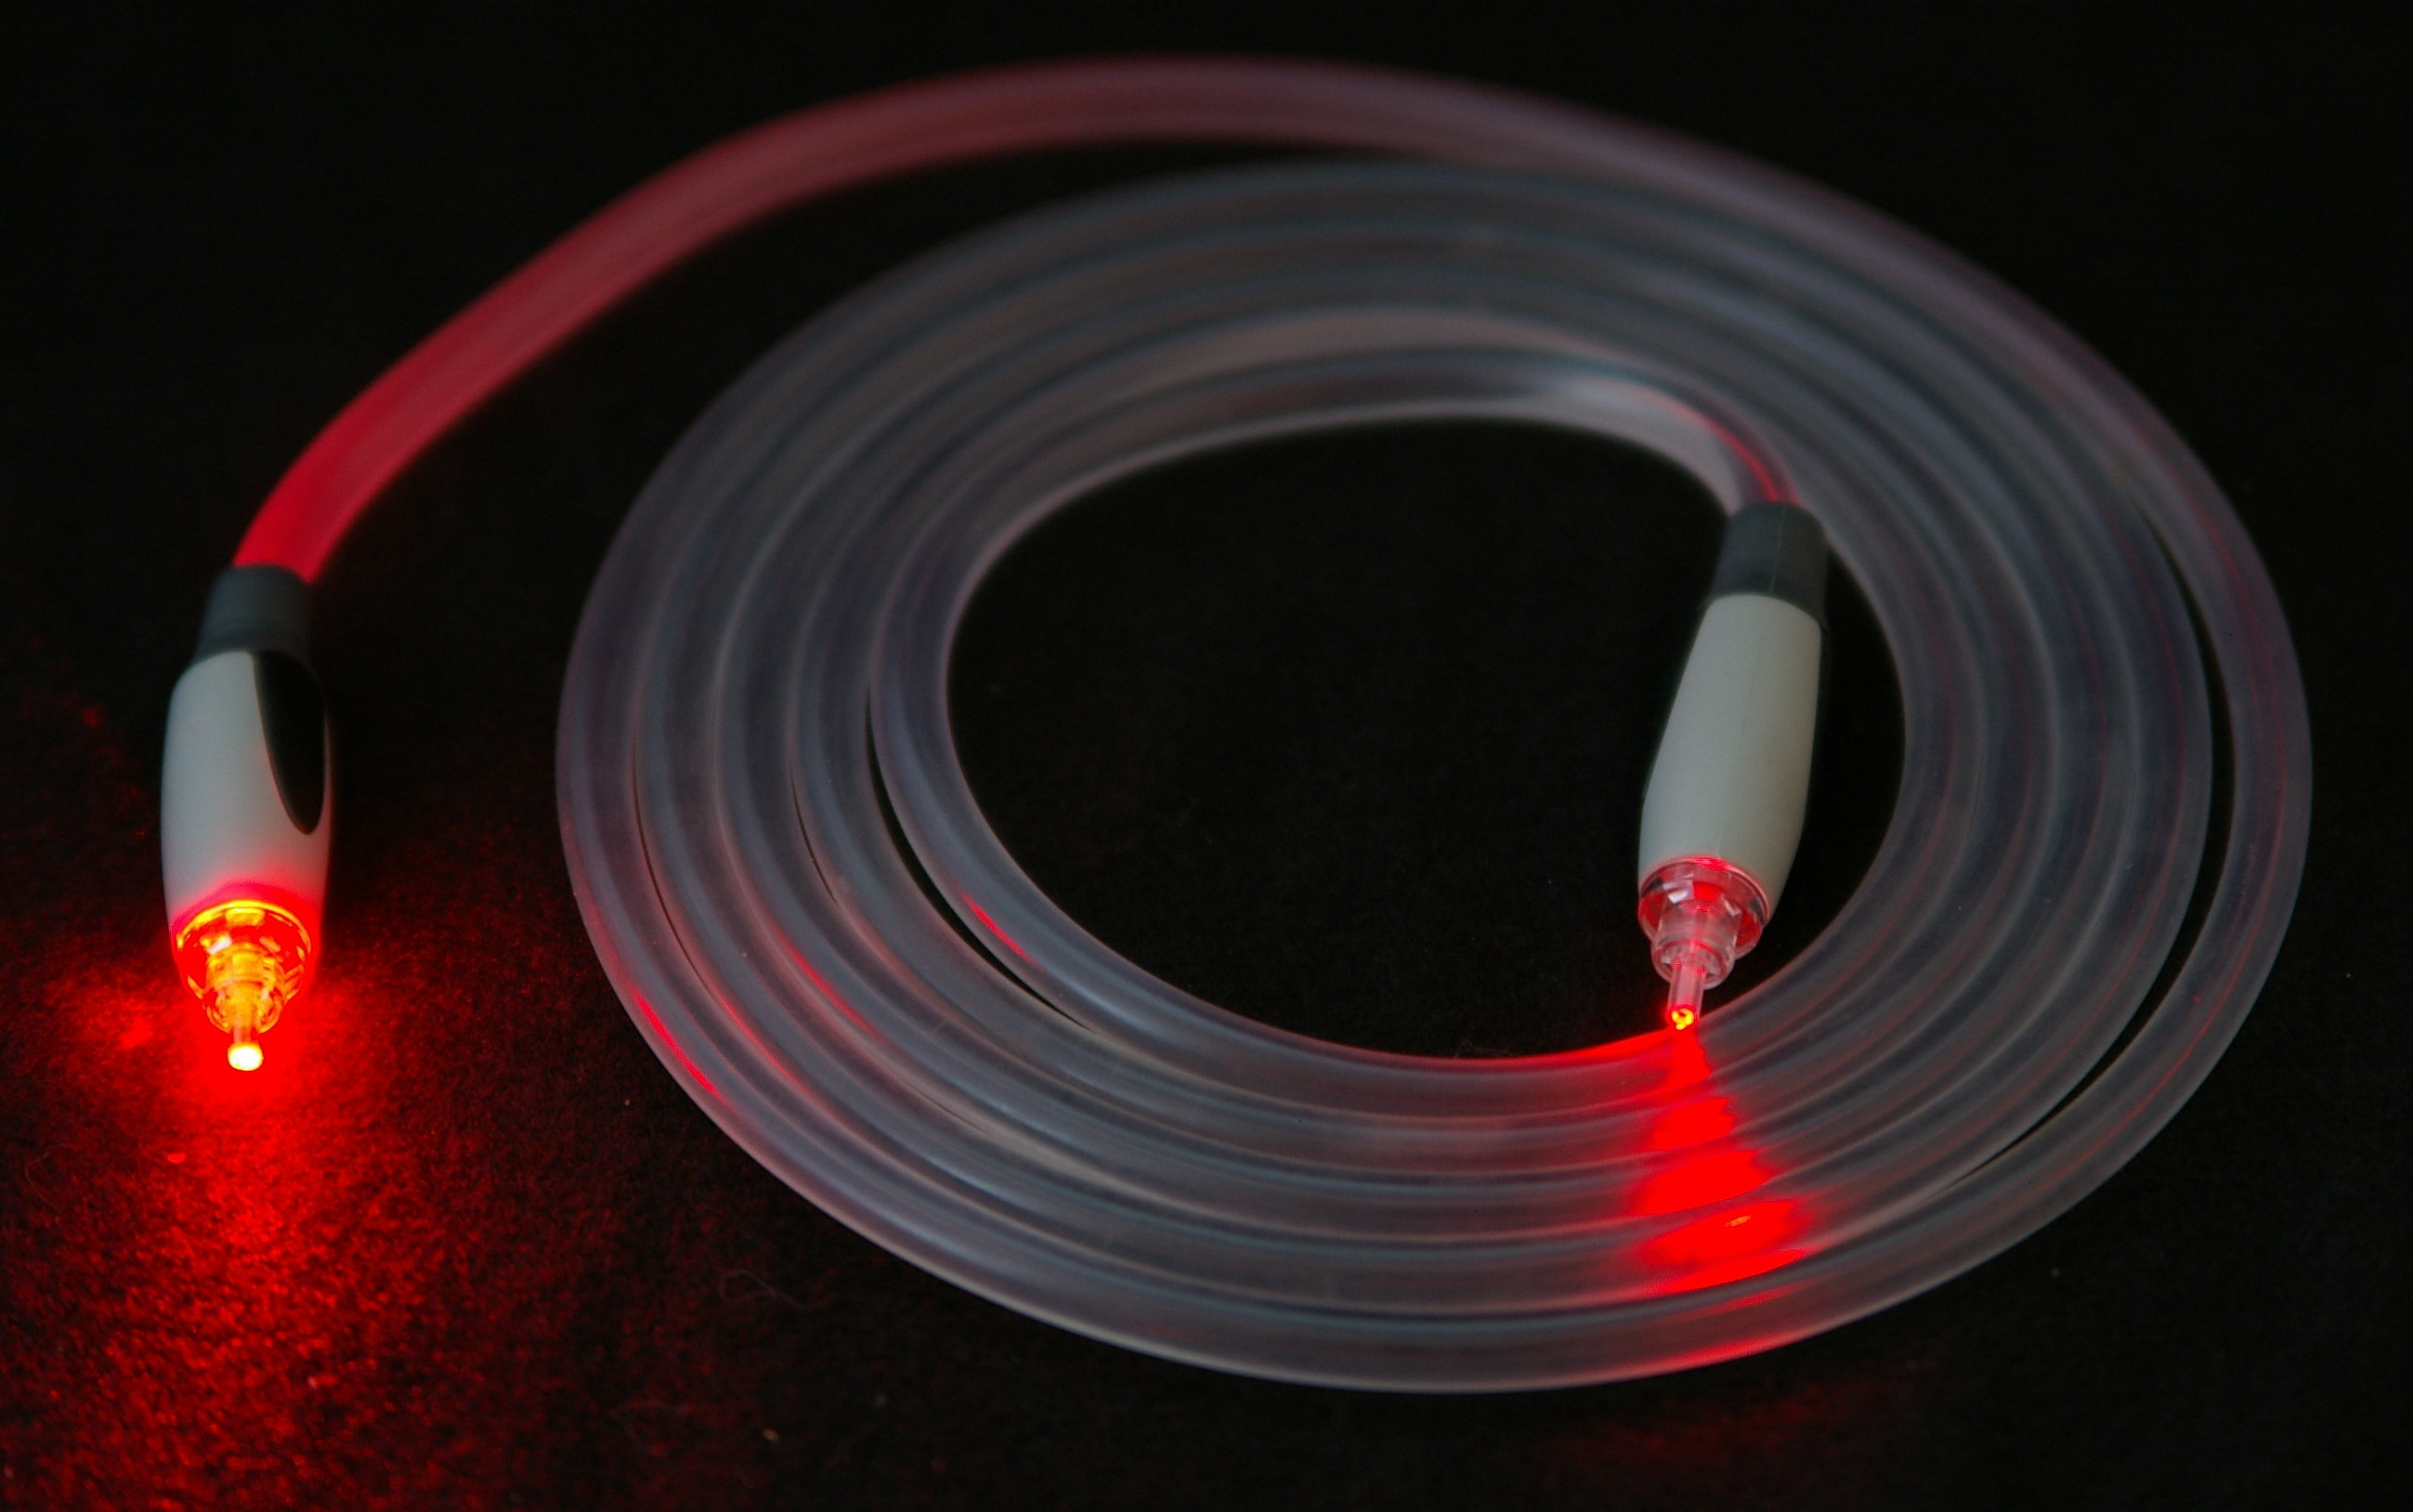
\includegraphics[width=4.3cm]{../physical/Fiber_optic_illuminated.jpeg}
}; \&
\node[draw,label={[credit]south:Dmitry G, CC BY-SA 3.0, via Wikimedia Commons},
      label={[type]north:bundle of wires}] (eth)  {
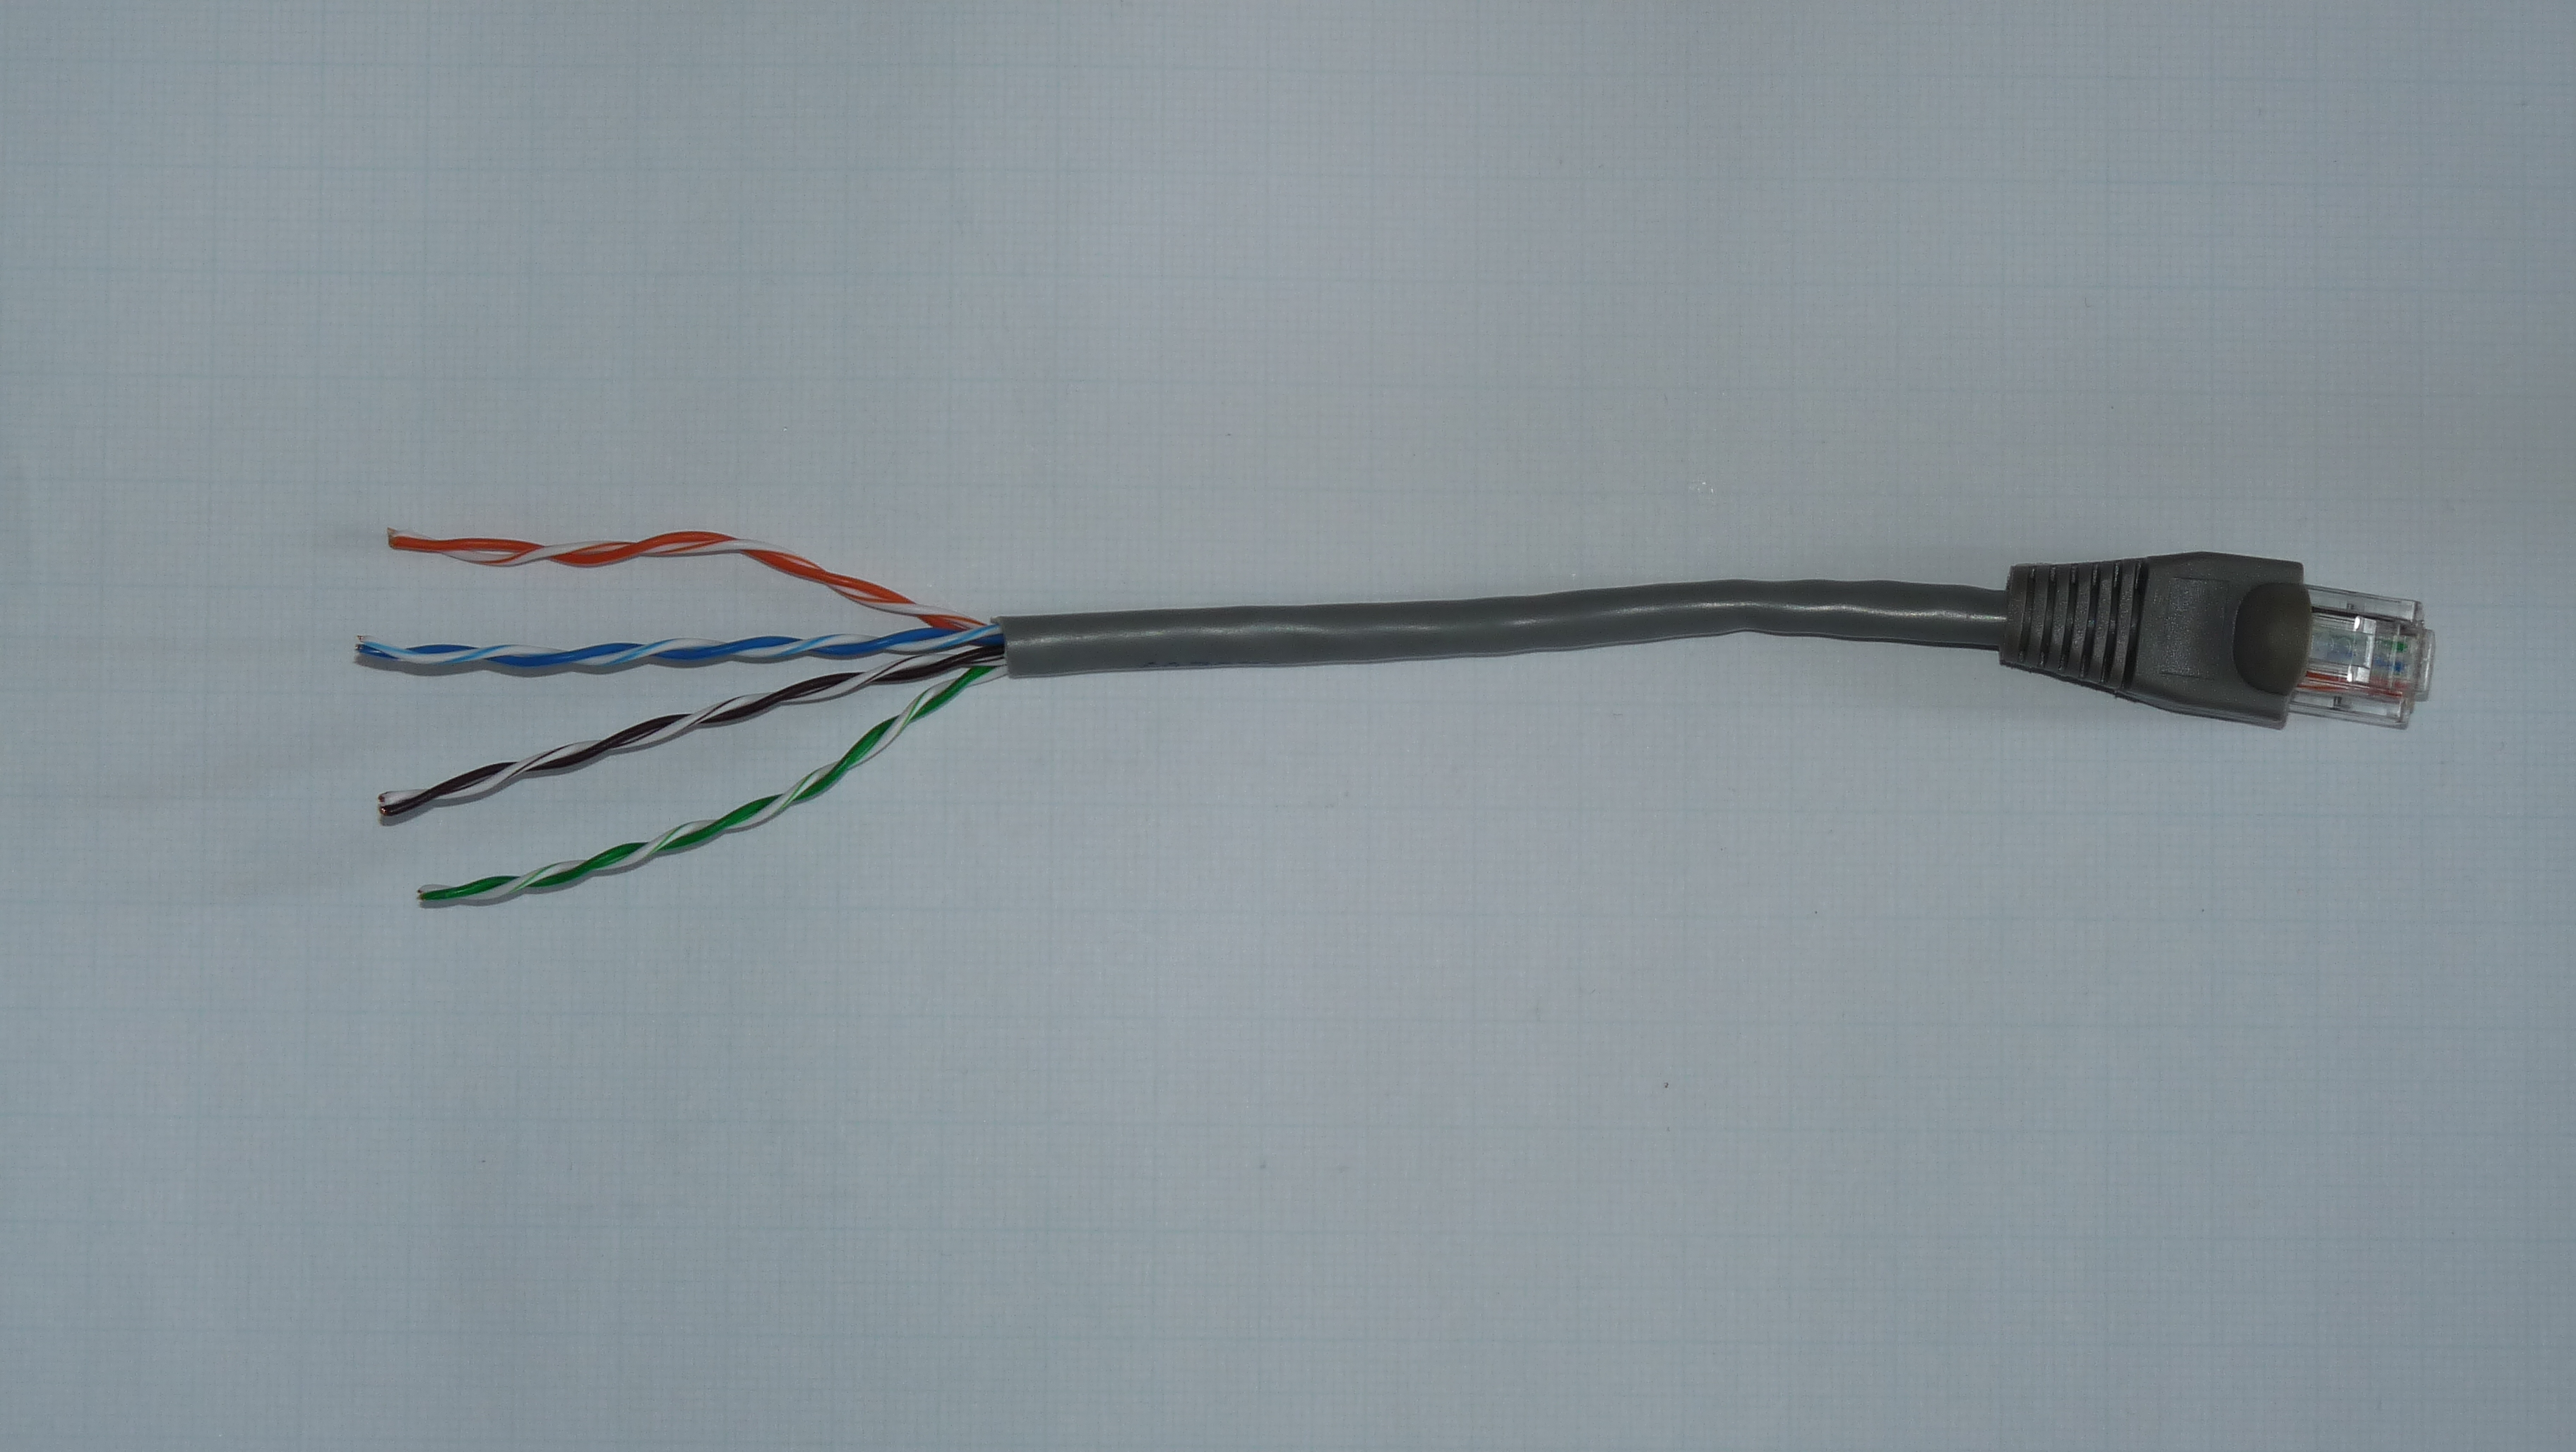
\includegraphics[width=4.3cm]{../physical/Ethernet_cable.jpeg}
}; \&
\node[draw,label={[credit]south:Adamantios, CC BY-SA 3.0, via Wikimedia Commons},
      label={[type]north:infrared through air}] (fso)  {
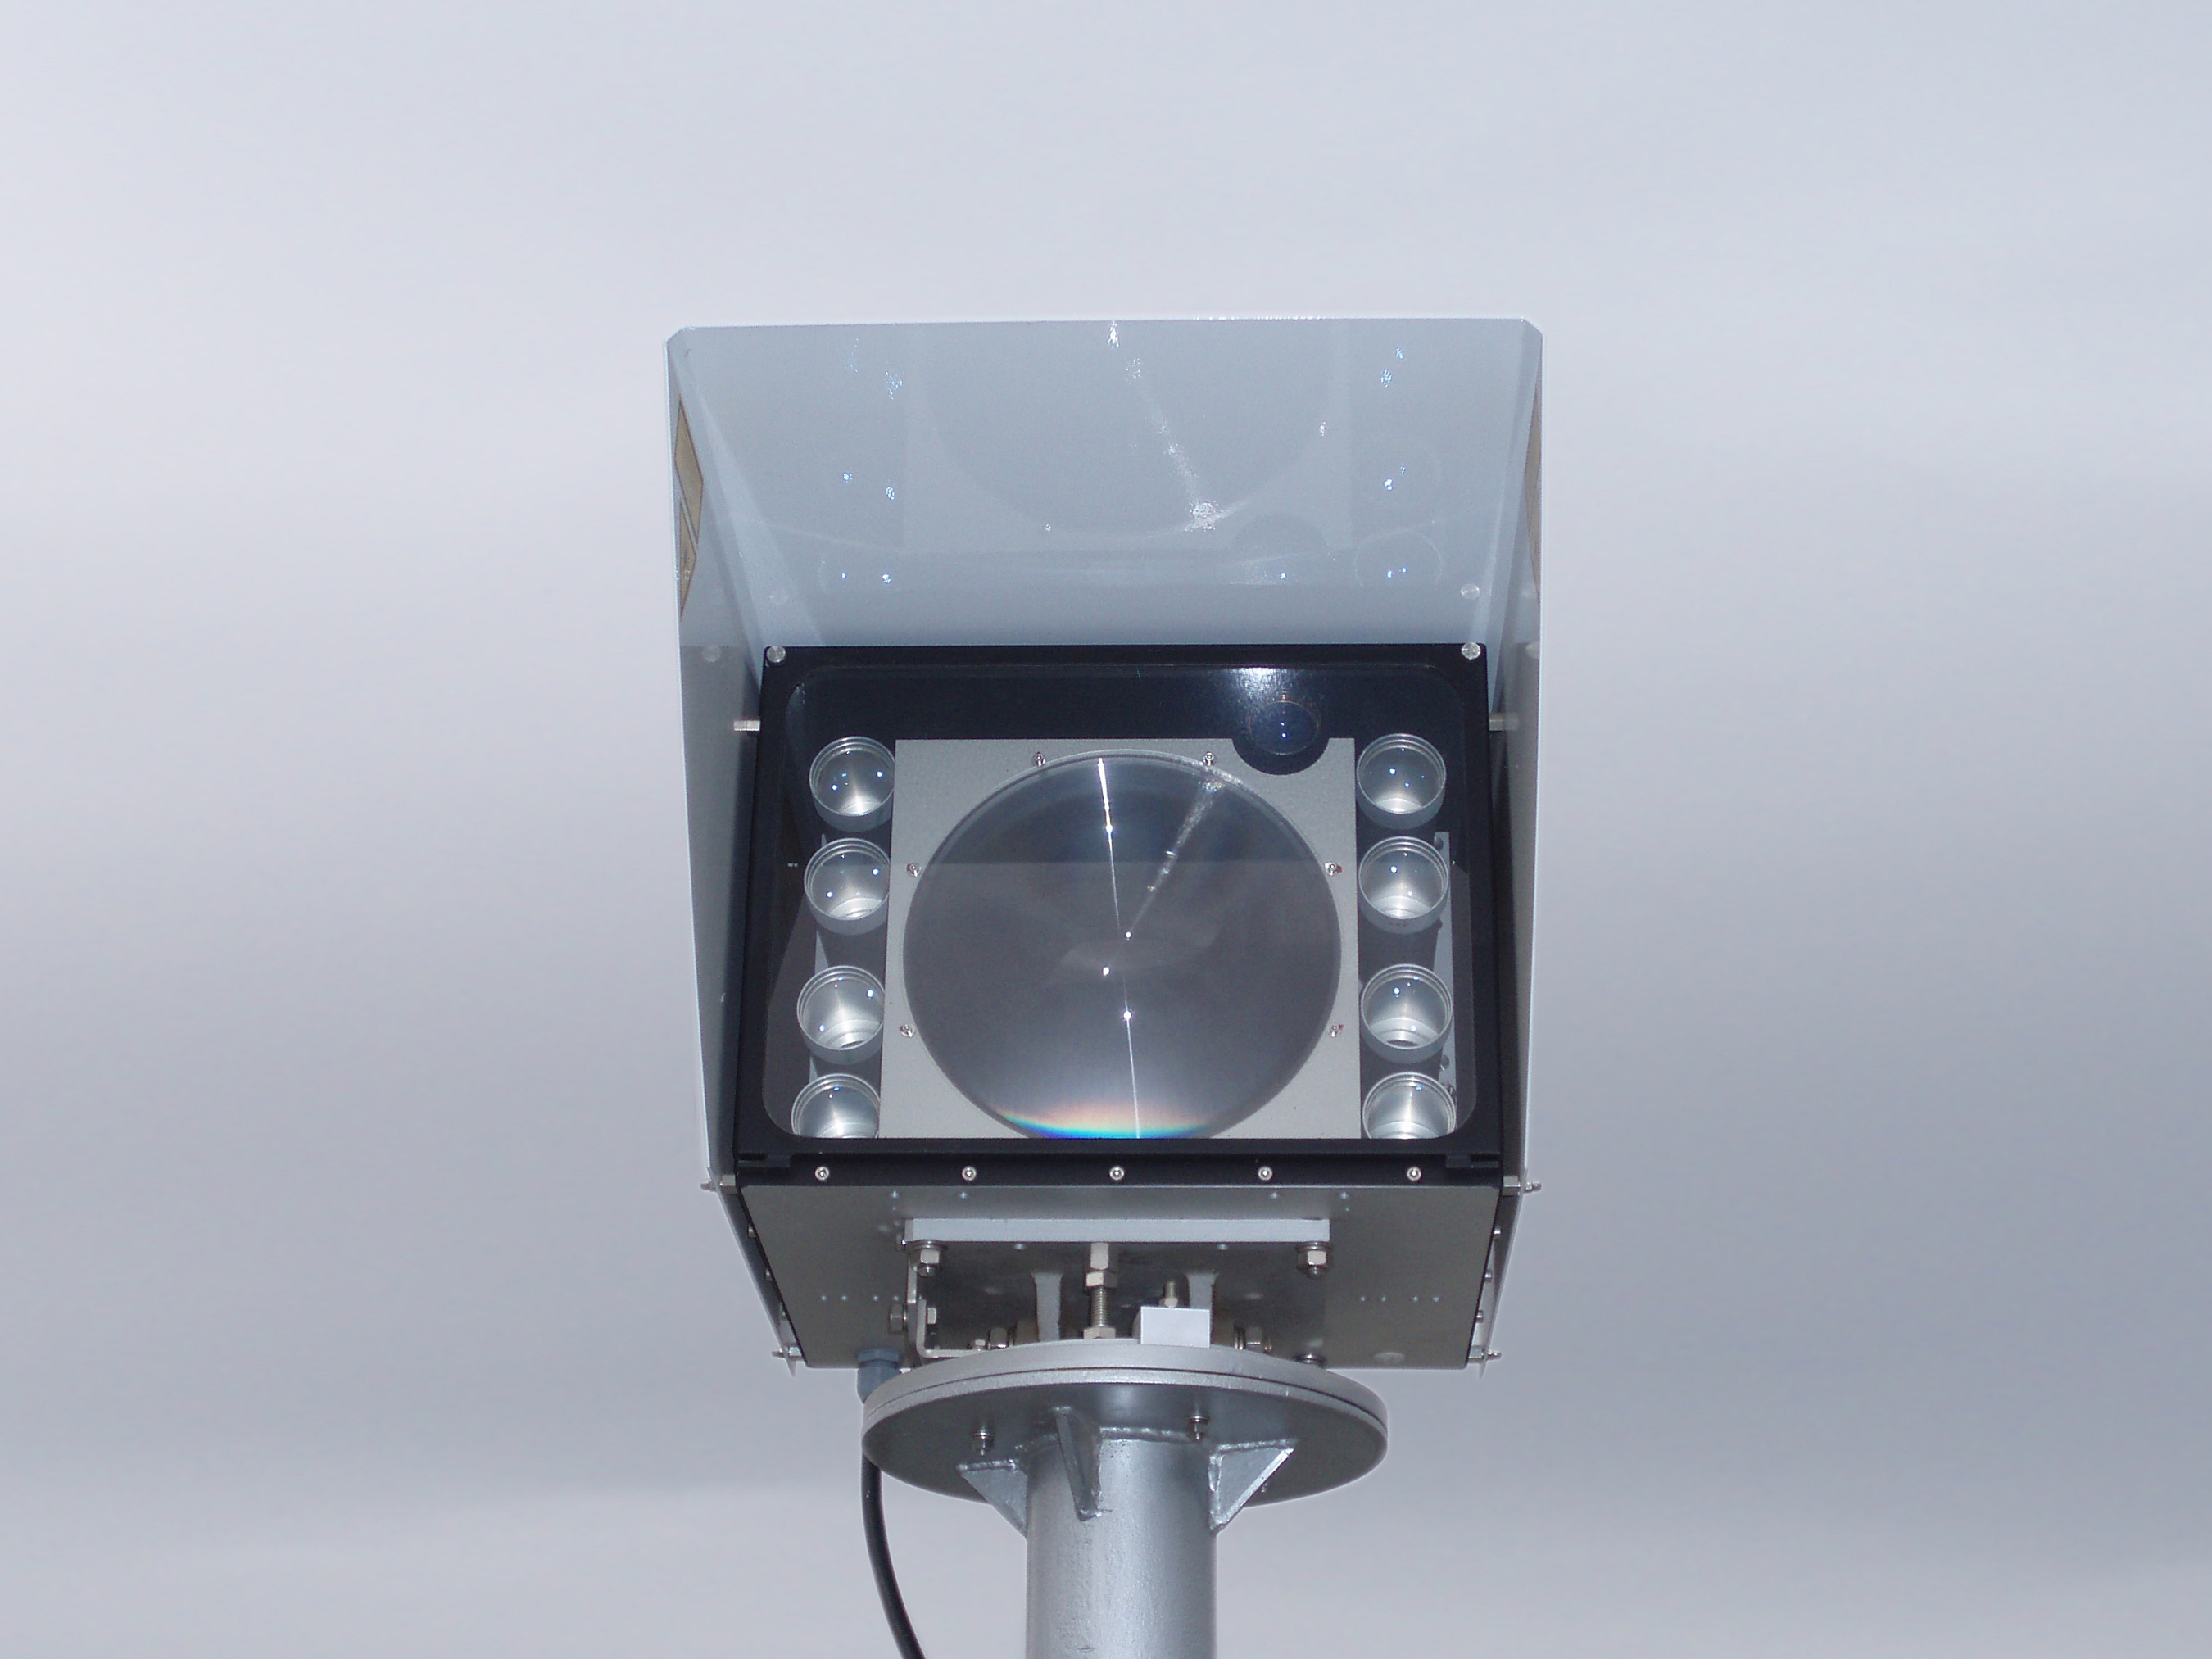
\includegraphics[width=3.7cm]{../physical/FSO-gigabit-laser-link-0a.jpeg}
}; \\
\node[draw,label={[credit]south:FDominec, CC BY-SA 3.0, via Wikimedia Commons},
      label={[type]north:single wire}] (coax)  {
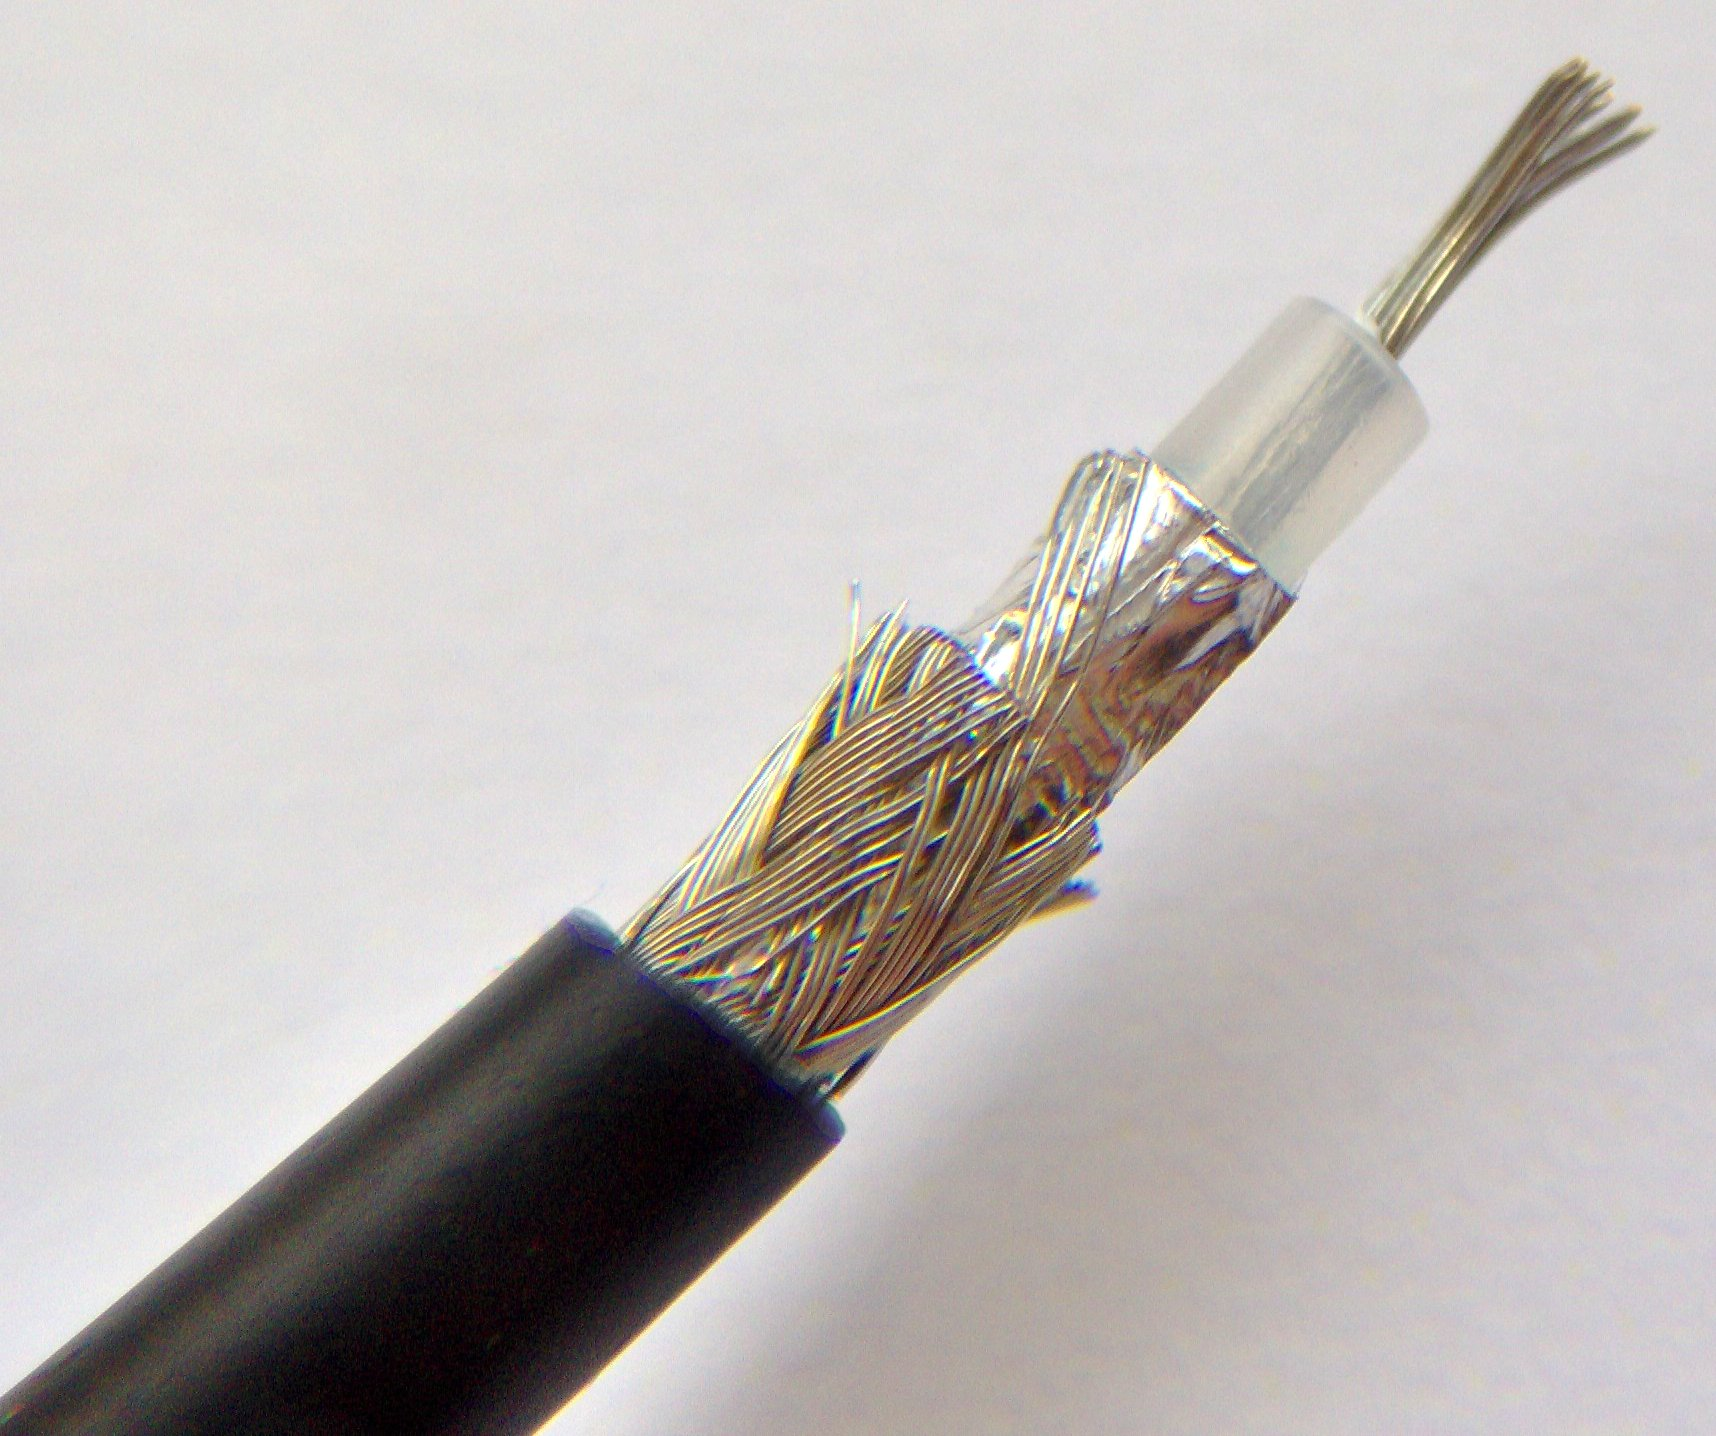
\includegraphics[width=3.3cm]{../physical/Coaxial_cable_cut.jpeg}
}; \&
\node[draw,label={[credit]south:Evan-Amos, via Wikimedia Commons},
      label={[type]north:radio}] (wifi)  {
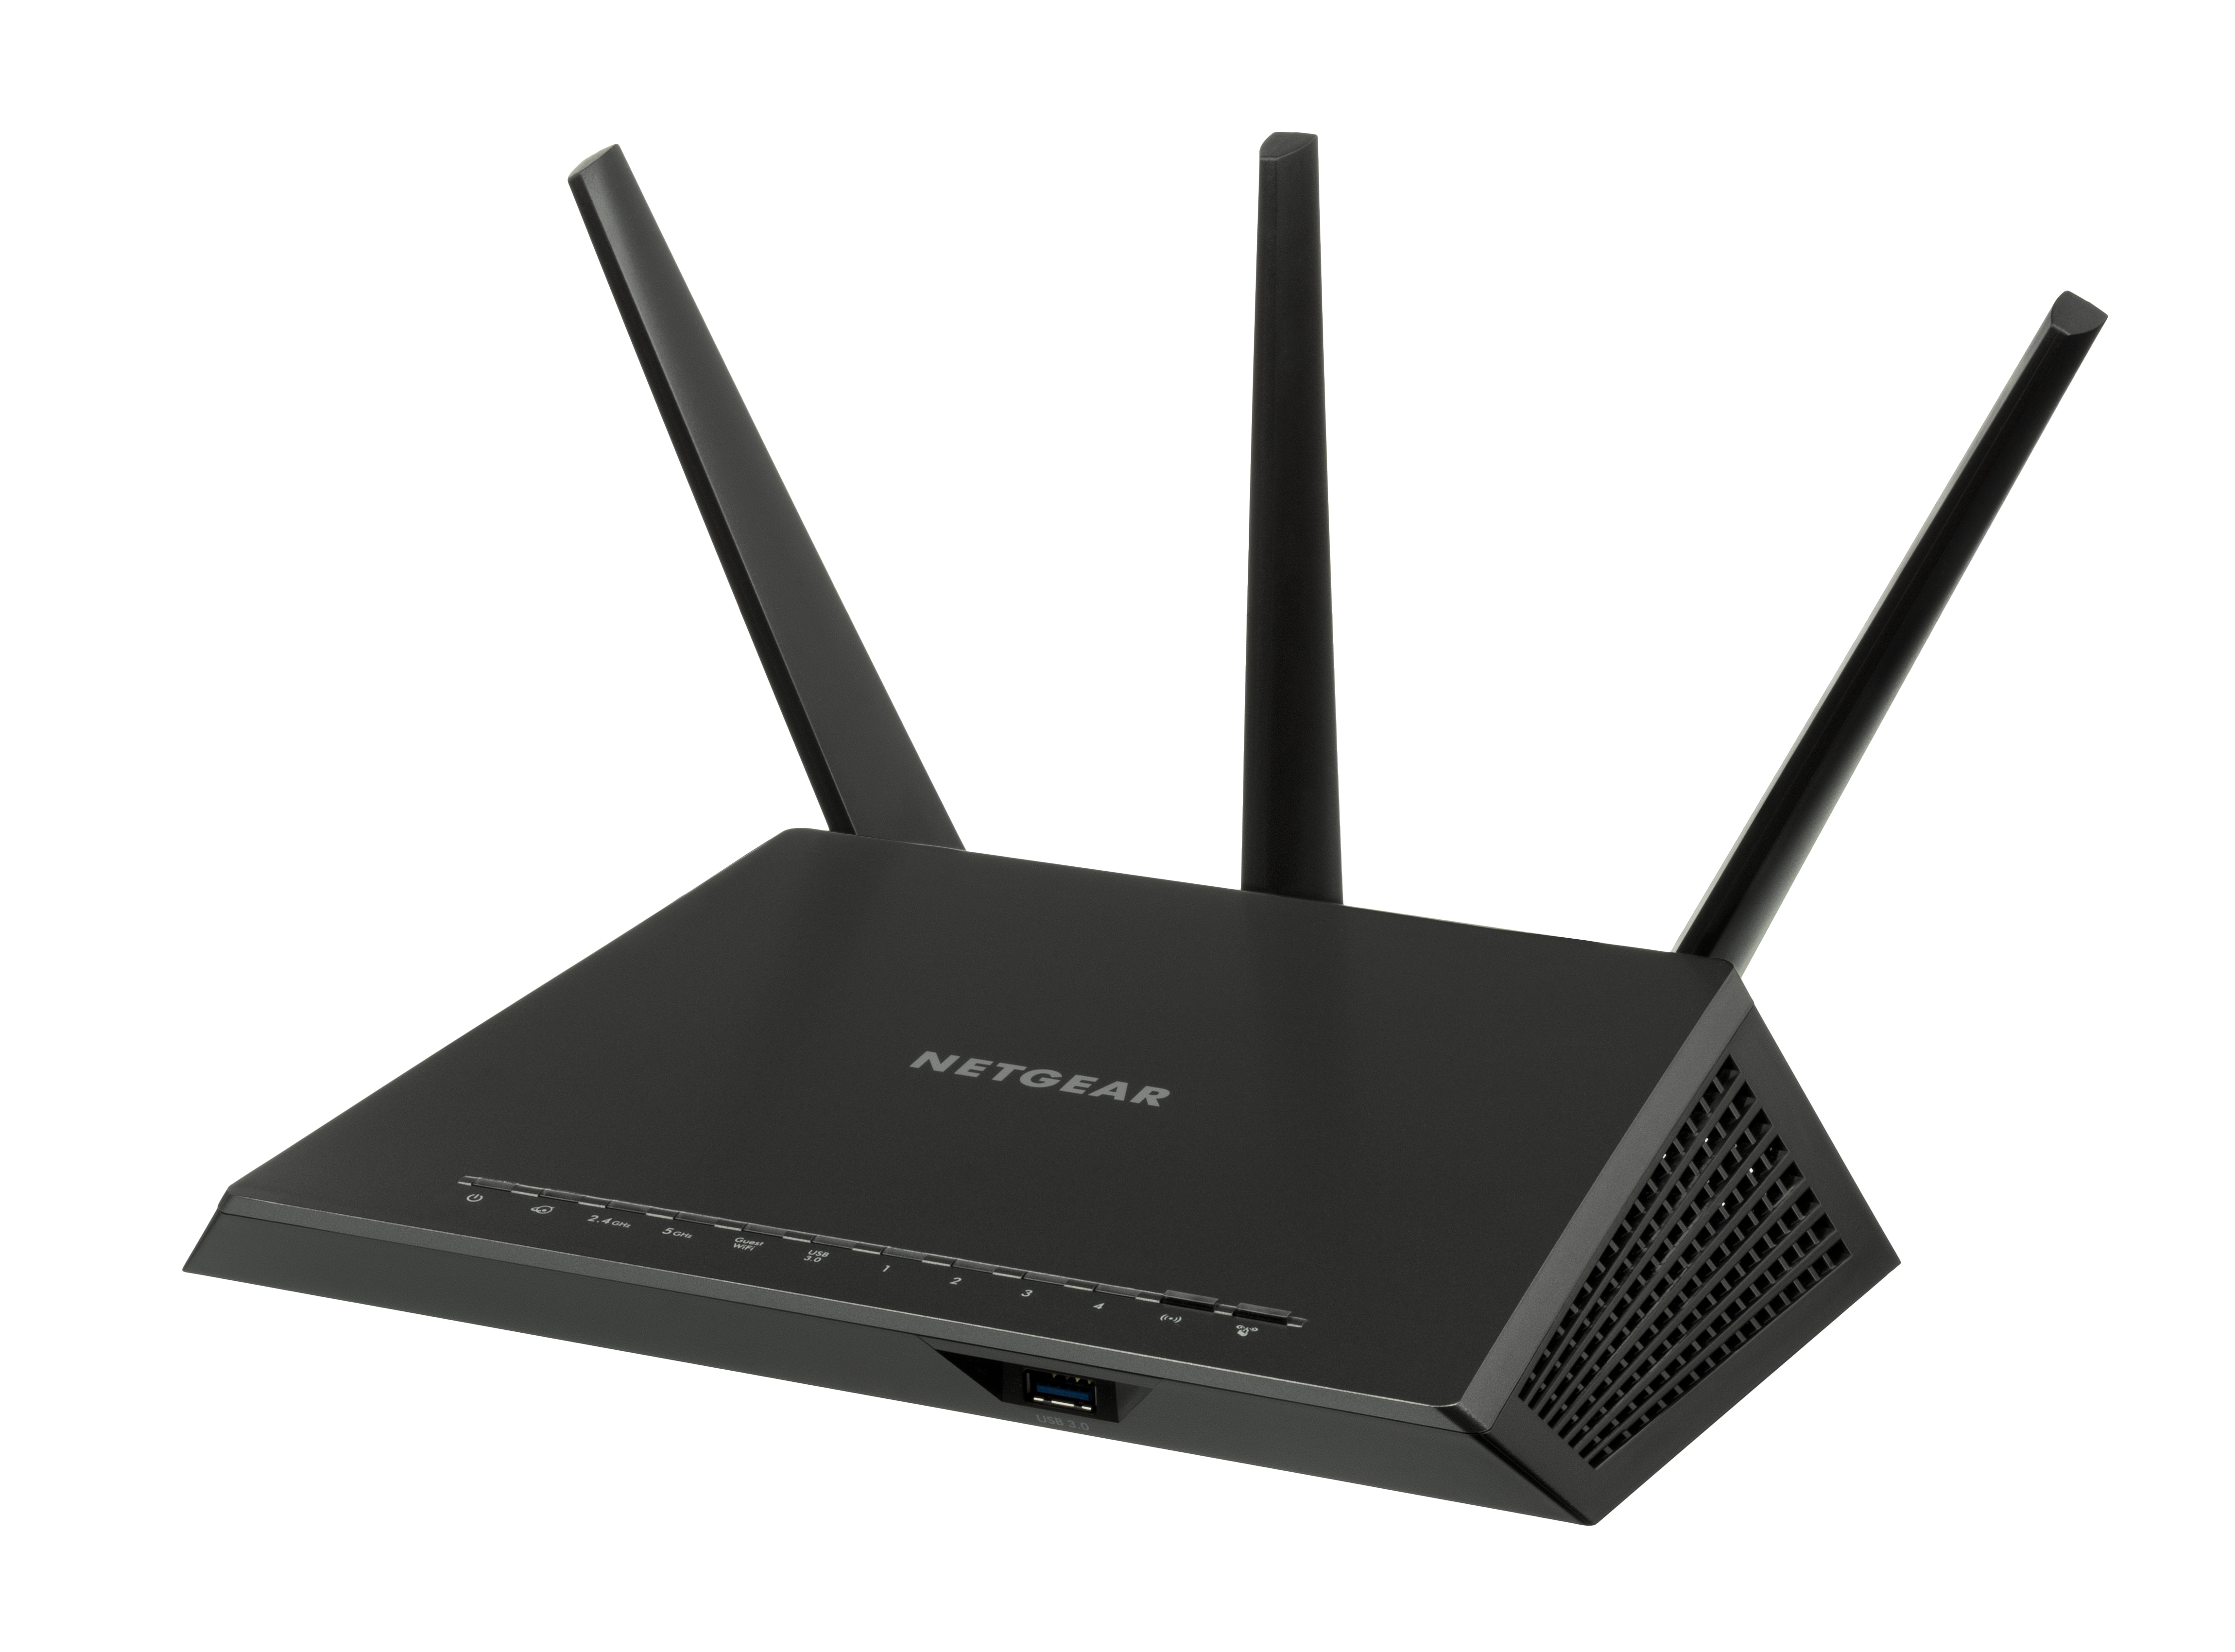
\includegraphics[width=3.7cm]{../physical/Netgear-Nighthawk-AC1900-WiFi-Router.jpeg}
}; \& \node[draw=none] (dotdot place) {}; \\
};
\node[draw=none,font=\Huge,anchor=center] (dotdot) at (wifi.east -| dotdot place.center){\ldots};
\end{tikzpicture}
\end{frame}
